% -*- mode: latex; mode: auto-fill; coding: utf-8; -*-

% What is meant by the simulation model
The \defit{simulation model} is here defined to be the fundamental components
driving the simulation. The fundamental components are responsible for
the user interaction, solving the system of equations and visualizing
the results in a three-dimensional scene. 
The following section will introduce the fundamental components of the
simulation model. We will elaborate on the responsibility of each component
and the technologies used.
%
An overview of the simulation model is illustrated in figure
\vref{fig:simulation_model}.  

\begin{figure}
  \centering
  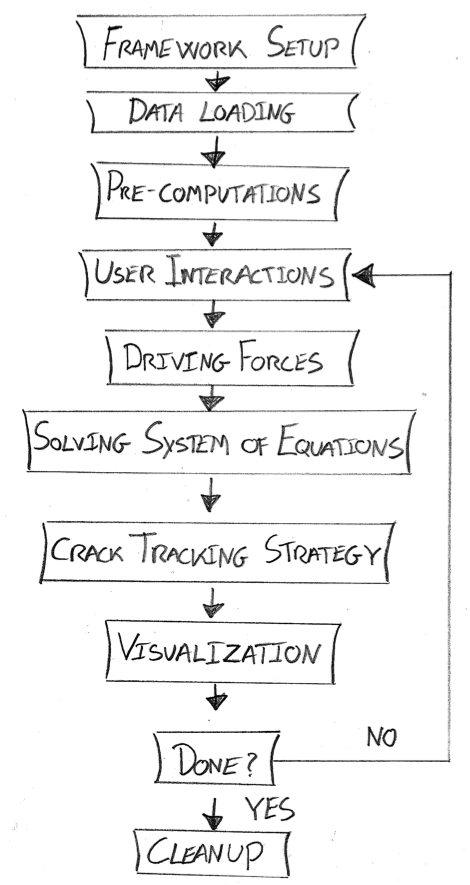
\includegraphics[width=5.8cm]{./images/simulation_model.png}
\caption{Overview of the simulation model.}
\label{fig:simulation_model}
\end{figure}

% briefly explain the figure
\subsection*{Framework Setup}
The simulator model is implemented using the
\openengine{} framework\refweb{http://www.openengine.dk}
which is a lightweight visualization framework with a small core and
an easy to use extension system. The framework is written
in C++\refweb{http://en.wikipedia.org/wiki/C++} and the build system
cmake\refweb{http://www.cmake.org/} makes is easy to build on Windows,
Linux and Mac OS X. The authors of this thesis are also the co-authors of
the \openengine{} framework so the choice was obvious. \\
 
The first step is to set up the \openengine{} framework. The framework
handles the main loop of the application. All components that need
process time must be inserted into the framework as modules. The modules will be
processed in a sequential manner in each main loop iteration. Setting
up the framework includes adding 
nodes to the scene graph, setting the position and orientation of the
camera, adding input handlers, and setting the path to
disk resources like models and textures.


\subsection*{Data Loading}
\label{sec:data-model}
Some resources have to be loaded from disk. The primary 
resource loaded is the solid model we are interested in
simulating. The solid model is loaded into memory using a TetGen
loader. TetGen\refweb{http://tetgen.berlios.de/index.html} is
an open source project capable of generating a tetrahedral mesh
from a surface representation of a solid model. 
% how is the solid represented in memory (solid - body - surface - vertexpool)  
%
The data model representing the model consists of a vertex-pool, a
surface mesh, and a body mesh. The vertex-pool is an one-dimensional
array containing vertices represented in global space as vectors.
Each component of a vertex vector is represteted as a single
precision floating point
number. The surface and body meshes are one-dimensional arrays
containing integer indices, pointing into the vertex-pool.
The surface mesh bundles three indices pointing to three vertices
in the vertex-pool defining one triangular face of the surface.
The body mesh bundles four indices pointing to four vertices
defining a tetrahedron.
%
The surface mesh is used during visualization while the body
mesh is used when solving the system equations and for
fragmentation.

\subsection*{Pre-computations}
\label{sec:precompuations}
The pre-computations are an important part of the Total Lagrangian Explicit
solver as explained in section \vref{sec:nodal_displacement}. The
equation for displacement as defined by \eqref{eq:displacement-vector-component-wise} on
page \pageref{eq:displacement-vector-component-wise} has been
simplified through pre-computation of the mass, the damping, and the
three matrices $A$, $B$, and $C$ as defined in equation
\eqref{eq:vector_component_abc} on page
\pageref{eq:vector_component_abc}. The pre-computations are essential
to the performance of the solver. By 
pre-computing as much as possible more resources are made available at run-time.
%
The shape function derivatives are an important part of the finite
element method and can also be
pre-computed. The shape function derivatives are precalculated as explained
in section \vref{sec:selecting_interpolation_function}.\\

Explicit time integration operators such as the central difference
method used is only conditionally stable. The main concern on the
approximating method is the fact that the error increases with the
time step size.
%Using the central difference method the approximation error has a
%growth of $\Delta t^2$.
It is essential to keep the time step size small or else the
approximation error will grow out of proportion causing numerical
instability.
%To determine how small the time step must be we must consider the
%geometry of the problem.
%When the time step size is small so is the error. 
%With a small enough size of the
%time step the error can be neglected. 
There is a complicated relation between the maximum allowed time step,
the geometry of the elements, and the material properties. To prevent
the explicit integration from becoming numerically unstable we must
determine the size of the critical time
step \citebook{page~654}{article:tled}: 

\begin{equation}
\label{eq:delta-t-cr}
  \Delta t_{cr} = \frac{L_e}{c}
\end{equation}

% \begin{equation}
% \Delta t_{cr} = \frac{L_e}{M}
% \end{equation}

where $L_e$ is the smallest edge length from the set of elements and
$c$ is the dilatational wave speed which describes how
fast sound travels through the material defined by:

\begin{equation*}
c = \sqrt{\frac{E(1-\nu)}{\rho(1+\nu)(1-2\nu)}}
\end{equation*}

% \begin{equation*}
% c = \frac{M}{\rho} 
% \qquad \Leftrightarrow \qquad
% \frac{1}{c} = \beta = \frac{\rho}{M}
% \end{equation*}
% $M$ is known as the P-wave modulus defined by:
% \begin{equation}
%   M = \frac{E(1-\nu)}{(1+\nu)(1-2\nu)}
% \end{equation}

where $E$ is Young's modulus, $\nu$ is Poisson's ratio and $\rho$ is
the density. These values are all material dependent and usually
determined by table look up. \\

% The
% critical time step $\Delta t_{cr}$ is predicted by a linear theory, but since
% we conduct non-linear analysis as explained in section
% \vref{sec:tled_solver} our stress-strain relation is non-linear. This
% means that the displacement increases drastically as the stresses and strains
% increases. Stability analysis conducted by \citebook{page~127}{article:miller}
% suggests a critical time step factor of $0.5$ to keep the
% displacements from exceeding the limit within reasonable
% deformations. If the deformation is extreme enough, dependent on the
% body being simulated, the integration scheme will still become unstable. \\
%
% neighbour list for the crack tracking
In order to improve the performance of the crack tracking algorithm, a
neighbouring list is pre-computed. Since it is a precondition that all
elements are interconnected, each element must have at least
one neighbour and maximum four. By pre-computing the neighbouring list
the problem of finding neighbouring elements reduces at run-time from an $O(n^2)$
to an $O(1)$ problem by table look up. \\

Finally the initial volume of each element is pre-computed. The
initial volume is used when calculating the nodal 
force contributions as explained in section
\vref{sec:nodal_force_contributions}.


\subsection*{User Interactions}
The user interaction is handled by the \openengine{} framework. The module
handling the user interaction is attached as a listener to the device
registering the input. The device could be a keyboard,
mouse, joystick, or haptic device. When input is registered all
attached listeners are notified and proper action is taken by
the receivers. Since the \openengine{} framework is single
threaded, the event queues are only flushed once during each main loop
iteration. The simulation must produce a minimum of 25 frames per
second in order to accommodate the demand for real-time
execution. Since each main loop iteration produces one frame the user
interaction will be handled with the frame rate.  


\subsection*{Driving Forces}
The initial state of the body is equilibrium. When there are no
external forces acting on the body there are no internal forces. As
explained in section \vref{sec:equilibrium-for-a-continuum} the body
is in equilibrium 
when the external forces equals the internal forces (equation
\ref{eq:pompe}). So in order for the system to react we have to apply
external driving forces. The driving force can be applied to nodes in the
entire domain, like the gravitational force would be, or it can be
applied to only parts of the domain. To affect the system we have
implemented different types of modifiers. The concept of modifiers and
the different types are explained in section
\vref{sec:modifiers}. Modifiers like the \defit{force 
  modifier} and the \defit{displacement modifier} change the
equilibrium of the system by adding external forces or by changing the
displacements, respectively.

\subsection*{Solving the System Equations}
The system equations must be solved in each iteration to constantly
converge towards equilibrium. The solving technique is explained in detail
in section \vref{sec:tled_solver}. The explicit solver
is a straightforward algorithm that in a fixed
number of steps calculates displacements as a result of the externally
applied forces. \\
% As mentioned in section
% \vref{sec:tled_solver} the solving technique is highly suitable for
% parallel execution, so each of the computational steps is performed on
% the GPU in separate kernels. In the source file
% \code{Physics\_kernels.cu} the main kernel responsible for determining
% each nodal force contribution is implemented. \\
%

As mentioned in the acknowledgement PhD student Karsten Noe
kindly shared his knowledge and prototype solver. The solver is
implemented in a straightforward manner according to the 
TLED article \citeabook{article:tled}. Instead of reimplementing his work
we incorporated and re-factored parts of the solver. We have
reused the pre-computation of the shape function but improved the
calculation of the nodal masses from an equally to a weighted
distribution. Furthermore we have improved the precision of the shape
function simply by increasing the floating point precision in the
intermediate calculations from single to double precision. We have
reused parts of the core matrix calculations, primarily the part where
quantities like the deformation gradient and the strain and stress
tensors are updated through matrix multiplications. We added all the
modifiers used for controlling the driving forces as elaborated in section
\vref{sec:modifiers}. The eigenproblem solver and all components
related to the crack tracking algorithm have been added. All debug and
visualization tools were implemented from scratch (elaborated in
chapter \vref{chapter:helper_tools}). 


\subsection*{Crack Tracking Strategy}
\label{sec:crack_tracking_strategy}
The \defit{crack tracking strategy} is responsible for determining
\defit{when} the material will crack and \defit{how} the crack will
propagate. The crack tracking strategy used here is
based on a local tracking scheme and the principle of maximum stress
direction as explained in section
\vref{sec:physics_crack_init}. Finding the maximum principal stress
means 
solving the eigenproblem as explained in section
\ref{sec:principal_values_and_directions}, therefore we need to
solve the eigenproblem for each tetrahedral element and compare the
maximum eigenvalue with the fracturing limit $\sigma_F$ defined for the
material. The eigenproblem is solved for each stress tensor in each
iteration, using a library. \\

\begin{center} 
\begin{minipage}[b]{\linewidth} 
\begin{pseudocode}[ruled]{Crack Tracking Algorithm}{ }
\label{pc:crack}
MaxStress \GETS 0\\
\FOREACH e \in E \DO
\BEGIN
  \mbox{solve eigenproblem for e}\\
  \IF eigenvalue > MaxStress \THEN
  MaxStress \GETS eigenvalue \\
\END \\ \\

\IF MaxStress>\mbox{$\sigma_F$} \THEN
\BEGIN
 \mbox{determine crack plane orientation from eigenvector}\\
 \mbox{add element $e$ to crack front set C}\\
\END \\ \\

\WHILE |C| > 0 \DO
 \BEGIN
 \mbox{lookup neighbouring elements}\\
  \mbox{determine crack plane from principal stress direction and
    cracked neighbours}\\
  \mbox{add uncracked neighbours intersecting crack plane to C} \\
  \mbox{remove cracked element from C}\\
  \END
\end{pseudocode} 
\end{minipage} 
\end{center} 

If the fracturing limit has been exceeded in one or more elements the
simulation is stopped and we switch from parallel to sequential
execution. The crack tracking algorithm is performed sequentially
since it would not benefit from a parallel approach because the crack
is propagating in a sequential manner. The element with the maximum
eigenvalue will be the first one to crack. Since the first element has
no cracked neighbours the orientation of the first crack plane is  
determined only by the maximum principle stress direction as explained in
section \vref{sec:crack_tracking_algorithm}. \\

In algorithm \vref{pc:crack} $E$ is the set of tetrahedral elements and
$C$ is the
crack front set. When the crack has been initiated the crack tracking
strategy will proceed by cracking neighbour elements until the failure
surface has propagated all the way through the solid object. The crack
tracking algorithm operates in a iterative way. When an element has been
cracked, all its neighbouring elements, intersecting with the crack
plane, are added to the crack front set. The crack front set is the
set of elements that will be cracked in the next iteration. As the
crack propagates the size of the crack front set usually increases
rapidly since most elements has more than one uncracked neighbour. But
when part of the failure surface reaches the surface of the solid object the
crack front set decreases. \\ 

\begin{figure}
  \begin{minipage}[b]{0.5\linewidth} % A minipage that covers half t‰‰he page
    \centering
    \subfloat[Initial crack plane]{\label{fig:crack_init}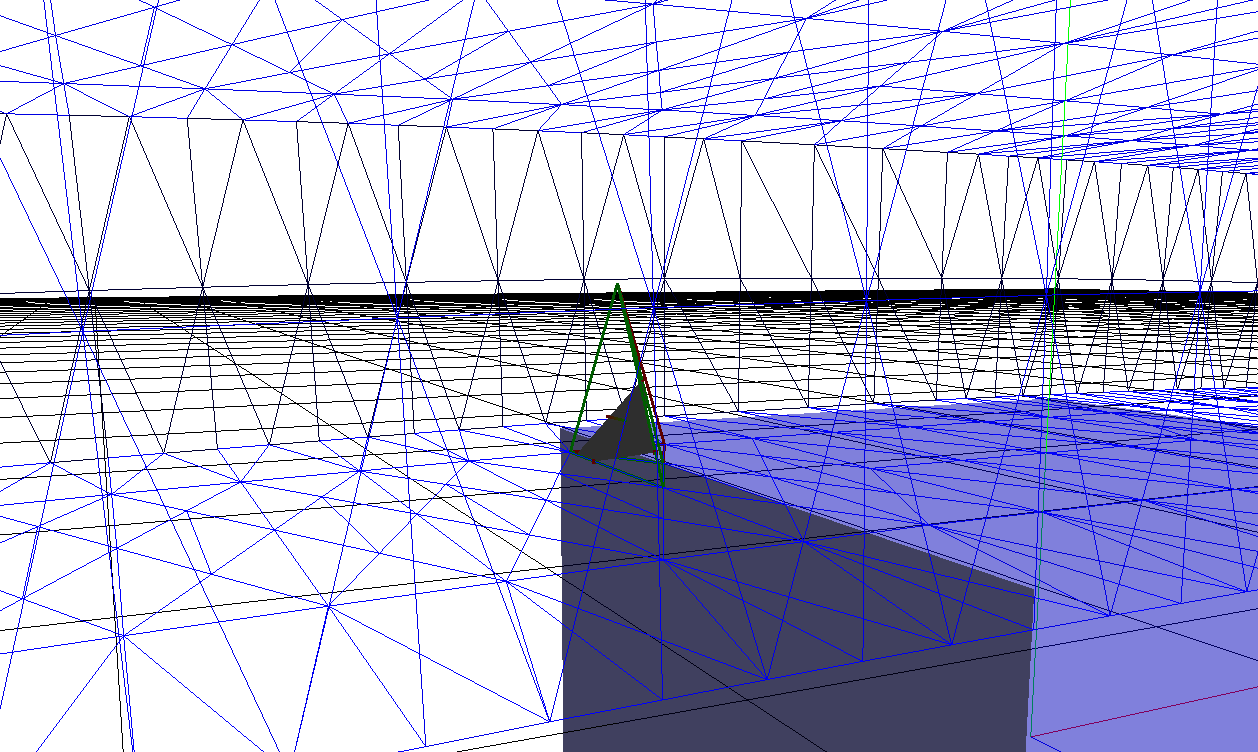
\includegraphics[width=70mm]{./images/simulation_model_crack_0.png}}
  \end{minipage}
  \hspace{0.5cm} % To get a little bit of space between the figures$
  \begin{minipage}[b]{0.5\linewidth}
    \centering
    \subfloat[First Neighbour element cracked]{\label{fig:crack_first}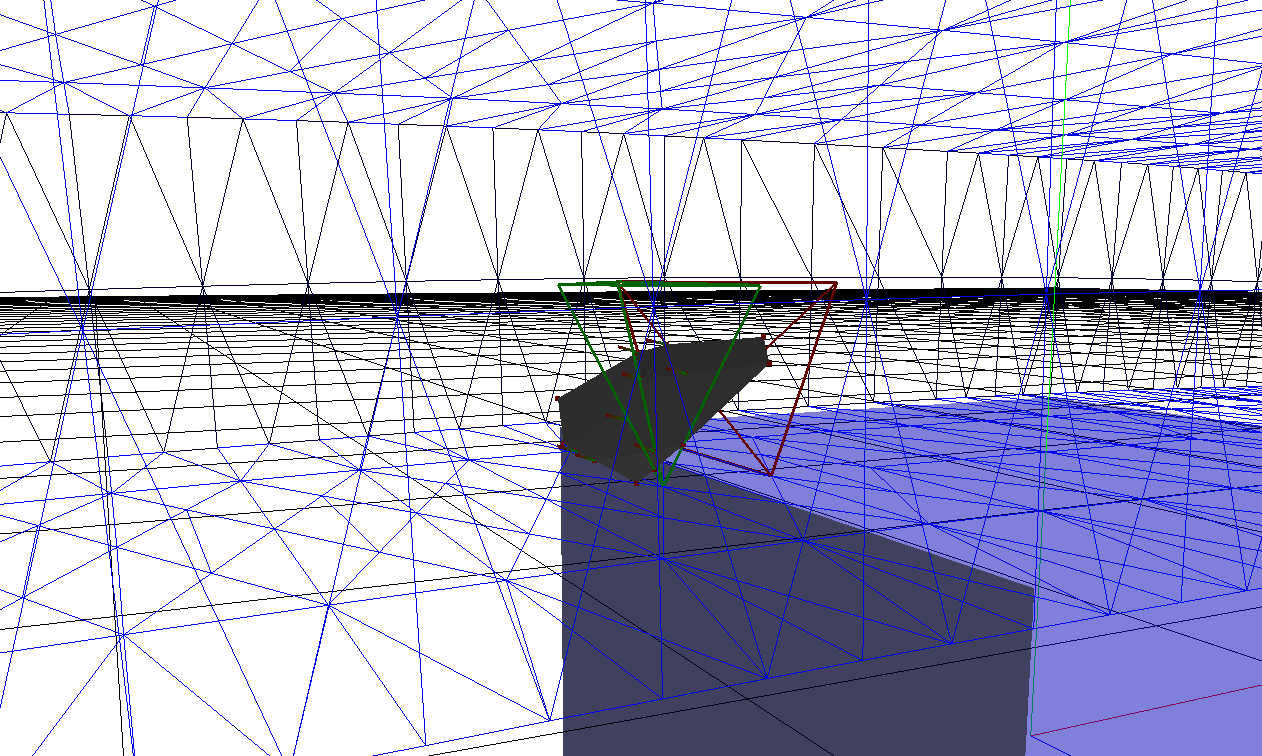
\includegraphics[width=70mm]{./images/simulation_model_crack_1.png}}
  \end{minipage}
  \newline
  \begin{minipage}[b]{0.5\linewidth} % A minipage that covers half the page
    \centering
    \subfloat[After the first iteration]{\label{fig:crack_second}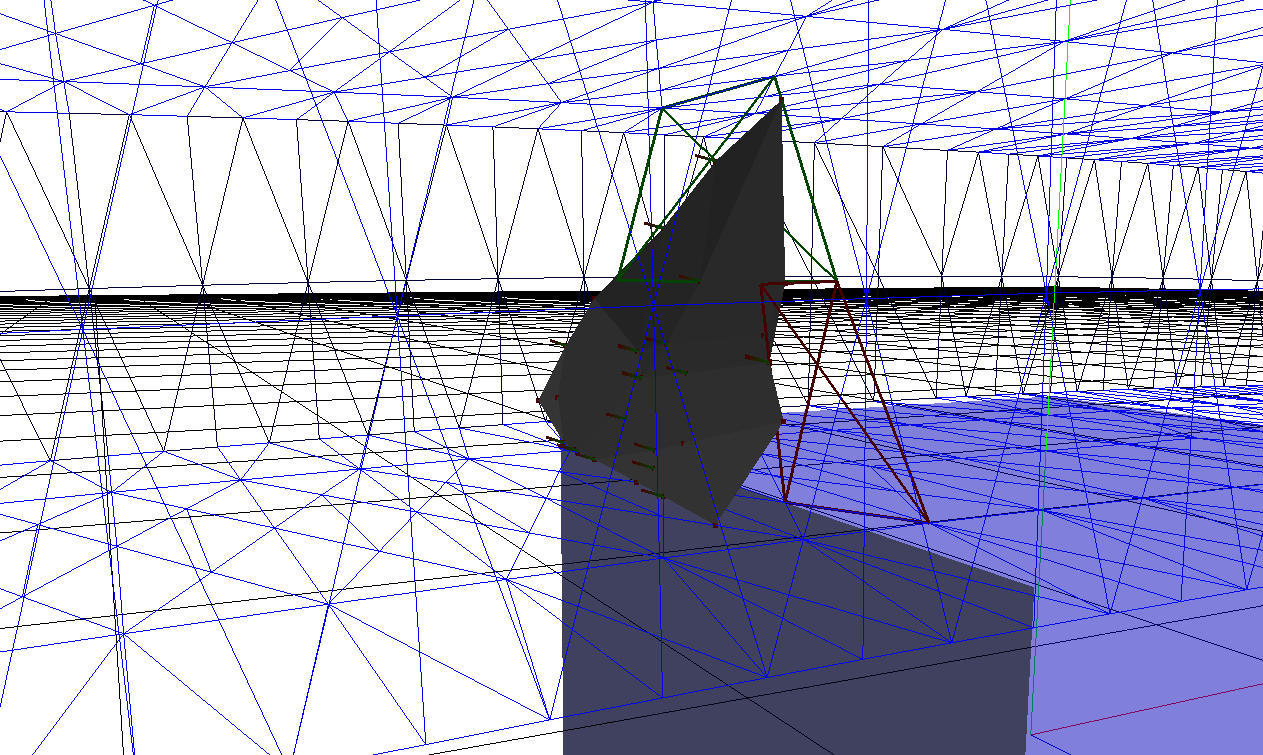
\includegraphics[width=70mm]{./images/simulation_model_crack_2.png}}      
  \end{minipage}
  \hspace{0.5cm} % To get a little bit of space between the figures
  \begin{minipage}[b]{0.5\linewidth}
    \centering
    \subfloat[Crack tracking done]{\label{fig:crack_done}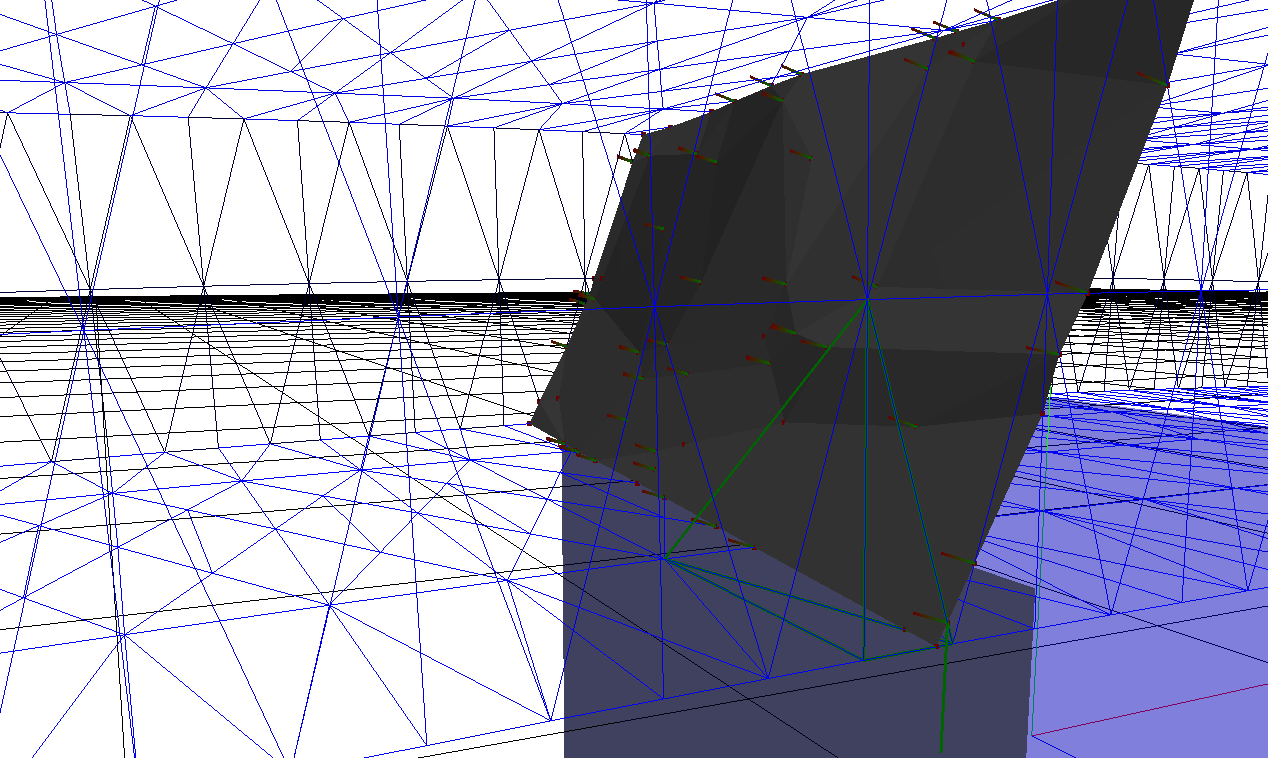
\includegraphics[width=70mm]{./images/simulation_model_crack_3.png}}
  \end{minipage}
  \caption{Crack propagation.}
  \label{fig:crack_tracking_in_progress}
\end{figure}

To illustrate the crack tracking algorithm consider figure
\vref{fig:crack_tracking_in_progress}. A concrete beam is
dropped on a solid box, gravity is the only external force
acting on the beam. Figure \vref{fig:crack_init} illustrates the
initial crack plane, where the orientation of the
plane is determined by the maximum principal stress direction.
%
Figure \ref{fig:crack_first} and \vref{fig:crack_second} illustrate
the propagation of the crack. Finally the failure surface has reached
the surface
of the object and the crack tracking has been completed as illustrated
in figure \vref{fig:crack_done}. 

\subsection*{Visualization}
The visualization is based
upon a scene graph and a renderer. The scene graph is a tree structure
of entities that can be visited breadth-first or depth-first by the
renderer as defined by the visitor pattern
\citebook{page~331}{book:gof}. The renderer is responsible for rendering 
the geometry on the screen, decoupling the rendering technology from
the representation of the geometry. The default renderer is
implemented using OpenGL\refweb{http://www.opengl.org/} due to its
cross platform libraries. 

% The system of equations are solved entirely
% on the GPU which means all the data resources are located in the VRAM
% on the graphics card. The visualization can easily be performed simply
% by setting up pointers to the resulting data already present on the
% graphics card. OpenGL handles this in a very elegant way where
% basically one line of code performs the actual rendering provided that
% the data is correctly aligned on the graphics card. 


\subsection*{Cleanup}
When the simulation is terminated the memory allocated must explicitly
be freed. This goes for the main memory as usual, but also for the
memory allocated on the graphics card. 

